%\{ {\it  sp1d\_ch3\_1.tex} \}

We now consider equation (\ref{poisson1}) in the viewpoint of
convergence having solution $u \in H^k(\Omega)= \{u|\sum_{|j|\le k
}\frac{d^j}{dx^j} \in L^2(\Omega) \}$.

Assuming a discretization on a uniform domain of equi-spaced
subintervals of size $h$, the general error estimate in the norm
$||\cdot||_{H^k(\Omega)}$ for the h-and p-type extension process
can be written as \cite{Karniadarkis}:

\begin{equation}
\label{hprelation}
||\epsilon||_{H^k(\Omega)} \le CH^{\mu-1}P^{-(k-1)}||u||_{H^k(\Omega)},
\end{equation}
where $\epsilon = u - u^{\delta}, \mu = \mbox{min}(k, P+1)$, and $C$ is independent of $h$, $P$ and $u$, but depends on $k$.

This means if a solution $u$ lies in  $H^k(\Omega)$ for sufficiently large $k > P+1$, then this error estimate shows that we can achieve exponential convergence as we increase the polynomial order P. Also in particular to h-extension process, the error respect to norm $||\cdot||_{H^1(\Omega)}$ satisfies:
\begin{equation}
\label{hrelation} ||\epsilon||_{H^1(\Omega)} \le K_1Ch.
\end{equation}
From \cite{Karniadarkis}, we see that the slope of the h-type
extension process is related to the minimum of $P+1$ and the
smoothness $k$ of the solution. Because our experiment involves
smooth solutions, we observe the slope of h-type extension graph
of errors to be very close to $P+1$.

\begin{figure}[h]
    \begin{center}
    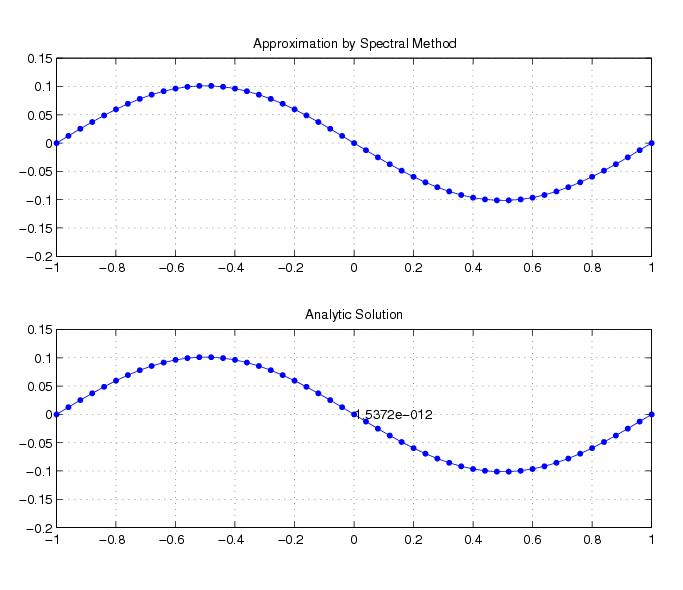
\epsfig{file = Doc-Report_Fwd1D/figs_dn/sinDN_O15.eps, width = 5cm}
    \caption{\label{sinsol1}Numerical and exact solution of equation (\ref{pois_sin1}) with polynomial order $P=15$}
    \end{center}
\end{figure}

\subsubsection {H/P Convergence Test for One-dimensional Solution}

\begin{figure}[h]
\begin{center}
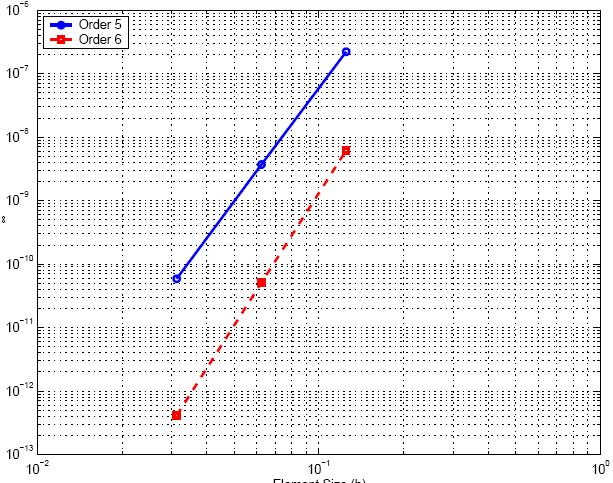
\epsfig{file = Doc-Report_Fwd1D/figs_dn/sinDNhconv.eps, width =8.3cm}
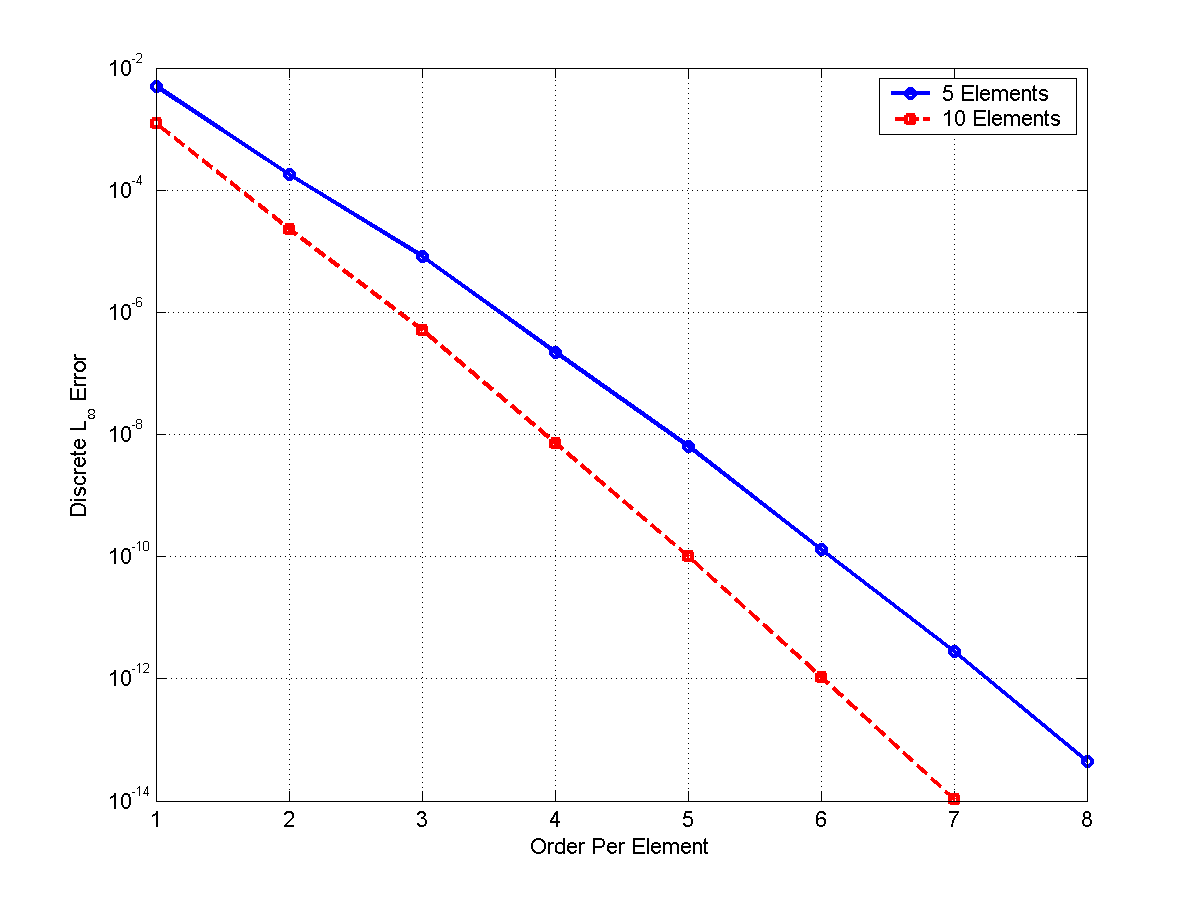
\epsfig{file =Doc-Report_Fwd1D/figs_dn/sinDNpconv.eps,width = 8.3cm}

\caption{\label{sinDNconv1} (Left) Convergence with respect to
discrete $L^{\infty}$ norm as a function of size of elements. This
test is performed using the h-type extension with polynomials of
order 3, 4, and 5 respectively. Error on the Log-Log axis
demonstrates the algebraic convergence of the h-type extension.
(Right) Convergence w.r.t. $L^{\infty}$ norm as a function of size
of polynomial order in semi-Log plot. This shows the exponential
convergence of p-type extension for smooth solution. The tests
were performed for p-type extension with element length $0.2$ and
$0.1$. }
\end{center}
\end{figure}
In this section we present the result of convergence in both $h$
refinement and $p$ refinement with the following steady-state
Poisson differential equation:
\begin{equation}
\label{pois_sin1} \frac{d^2}{dx^2} u(x) = \sin(\pi x),
\end{equation}
for all x in $[-1, 1]$ with zero Dirichlet and Neumann boundary
conditions.


For comparison, the numerical and exact solutions are depicted in
figure (\ref{sinsol1}).

\begin{enumerate}

\item {Convergence of h-type extension for equation (\ref{pois_sin1})}

This test seeks to establish the relation between size of element
and the accuracy of approximation. Utilizing equi-distance
elements, we investigate error. As shown in Figure
(\ref{sinDNconv1}), as elements decrease in size, the accuracy of
the solution improves.

As we see the relationship (\ref{hrelation}) in the theory, the
slope of convergence graph should exhibit slopes of slope 4, 5,
and 6 for the polynomial orders 3, 4, and 5, respectively. The
exact outcome is shown in left table of Table (\ref{hconv2t1}).

\item {Convergence of p-type extension for equation (\ref{pois_sin1})}

Since the exact solution is an infinite sum of polynomial
function, finite order interpolating trial functions cannot reach
ideal convergence. It is also apparant that the convergence will
stagnate before the error reaches machine precision, shown in
right figure of Figure (\ref{sinDNconv1}), the experimented
results support the behavior described in equation
(\ref{hprelation}).

\end{enumerate}

\begin{table}[h]
\centering \caption{\label{hconv2t1} This table shows the
convergence of h-type (left) and p-type (right) resolution control
done above Figure (\ref{sinDNconv1}). Observe that the slopes of
each order $P$ is $P+1$. }
\begin{tabular}{|c|c|c|} \hline
    Polynomial order&Error($L^{\infty}$)&Slope   \\ \hline \hline
    3&$1.1620e-012$ &$4.0024$ \\ \hline
    4&$4.6629e-014$ &$4.9877$ \\ \hline
    5&$9.7367e-014$ &$5.9775$ \\ \hline
\end{tabular}
\hspace{.5in}
\begin{tabular}{|c|c|} \hline
    &\multicolumn{1}{|c|}{Error}\\
    \raisebox{0.5\baselineskip}%
    {Element Size}&($L^{\infty}$) \\ \hline \hline
    0.2&$8.3267e-016$  \\ \hline
    0.1&$6.6613e-016$  \\ \hline
\end{tabular}

\end{table}
